\section{Gastos autônomos nos modelos de crescimento}\label{SecAutonomos}

Até então, pode-se dizer que a teoria do crescimento liderado pela demanda enfrentava um dilema. Não conseguia conciliar estabilidade, distribuição funcional da renda exógena e grau de utilização da capacidade produtiva igual ao normal/planejado, aparentando uma trindade impossível do crescimento, conforme pode ser visto no diagrama \ref{diagrama}\footnote{Este diagrama é inspirado no ``trilema'' do crescimento apresentado por \textcite{cesaratto_neo-kaleckian_2015}.}.
Essa trindade impossível se mostrou falsa com o desenvolvimento do supermultiplicador sraffiano (SMS).


\begin{figure}[htb]
	\caption{Trindidade ``impossível''}
	\label{diagrama}
	\begin{center}
		\resizebox{0.45\textwidth}{!}{%
			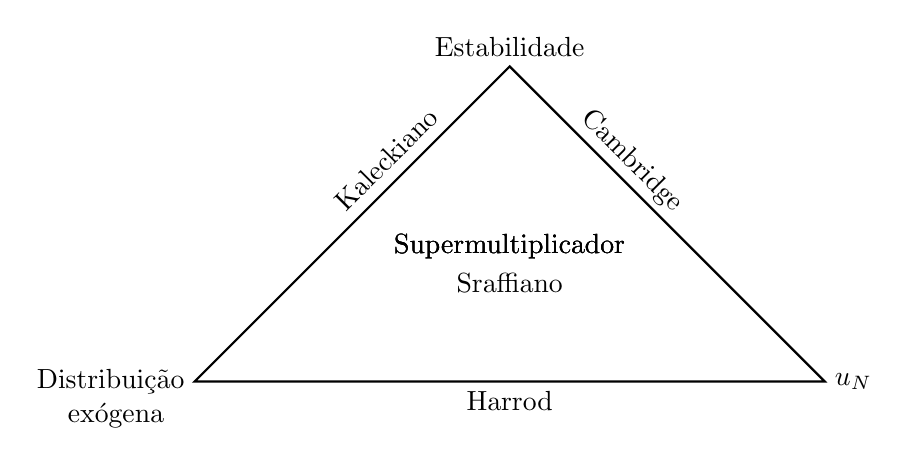
\begin{tikzpicture}[thick]
			\path[draw] (-4,0)  coordinate [label= left:Distribuição] (A)
			
			-- ( 0,4)  coordinate [label=above:Estabilidade] (C)
			-- ( 4,0)  coordinate [label=right:$u_N$] (B)
			-- cycle;
			\foreach \point in {A,B,C}
			\draw
			-- (0,2) node[anchor=north]{Supermultiplicador};
			\draw
			-- (-5,-0.15) node[anchor=north]{exógena};
			\draw
			-- (0,1.5) node[anchor=north]{Sraffiano};
			\draw
			-- (-1.75,3) node[anchor=north, rotate=45]{Kaleckiano};
			\draw
			-- (1.75,3) node[anchor=north, rotate=-45]{Cambridge};
			\draw
			-- (0,0) node[anchor=north]{Harrod};
			\end{tikzpicture}
		}
	\end{center}
	\caption*{\textbf{Fonte:} Elaboração própria}
\end{figure}

No entanto, da revisão da literatura verifica-se que tal mérito não se restringe ao SMS uma vez que uma vertente kaleckiana tem incluído tais gastos por meio do princípio do ajuste do estoque de capital no \textbf{longo prazo}.
Sendo assim, uma vez esclarecidas algumas das controvérsias em relação a autonomia dos gastos, é possível avançar em direção a um mapeamento de uma possível convergência entre os modelos sraffianos do tipo supermultiplicador e os modelos kaleckianos (seção \ref{Hibridos}) e então selecionar o caminho a ser seguido (seção \ref{Medium}).

\subsection{Um breve mapeamento da fronteira heterodoxa}
\label{Hibridos}


Ao longo desta seção, serão mapeados os modelos de crescimento, 
sejam eles kaleckianos ou sraffianos, liderados pelos gastos autônomos não criadores de capacidade produtiva ao setor privado. Isso não implica que são os únicos modelos com gastos autônomos, mas sim, que são os modelos em que a participação destes gastos não converge a zero\footnote{
	No que diz respeito ao consumo financiado por crédito, por exemplo, destacam-se os trabalhos de \textcite{dutt_maturity_2006}, \textcite{palley_inside_2010} e \textcite{hein_finance-dominated_2012}.
	No entanto, esses autores trabalham no arcabouço kaleckiano básico. Por isso, a estabilidade só é garantida se o consumo financiado por crédito a crescer a mesma taxa que a acumulação --- ou seja, este componente do consumo não pode ser tratado como de fato um gasto autônomo.
	%Diante desta limitação, \textcite{pariboni_household_2016} argumenta que os gastos autônomos desempenham um papel passivo e sugere uma alternativa a partir do supermultiplicador sraffiano. 
}.
Dado que estes modelos partem do fechamento do supermultiplicador sraffiano no longo prazo, os resultados esperados são: (i) mudanças na distribuição de renda não afetam a taxa de crescimento do produto; (ii) o mesmo vale para as alterações na propensão marginal propensão a poupar; (ii) convergência do grau de utilização ao normal; (iv) taxa de crescimento da economia converge à taxa dos gastos autônomos.
Sendo assim, as especificidades de cada modelo serão explicitadas somente se os resultados anteriores se alterarem de modo que serão analisadas as implicações da inclusão dos referidos gastos autônomos na medida que contribuam para os objetivos dessa pesquisa.
%Para manter a comparatividade entre os modelos apresentados, serão realçados alguns dos resultados de \textbf{longo prazo}, são eles: (i) mudanças na distribuição de renda; (ii) alterações na propensão marginal propensão a poupar; (ii) convergência do grau de utilização ao normal; (iv) aumento da taxa de crescimento dos gastos autônomos. Por fim, as variáveis serão adaptadas de modo que $\gamma$ é o componente autônomo do investimento,  $z$ é a participação dos gastos autônomos ($Z$) na renda que crescem a taxa $g_Z$.
Feitas essas ressalvas e seguindo a tipologia de \textcite{cesaratto_technical_2003} e a categorização de \textcite{serrano_sraffian_1995}, tais gastos autônomos são: (i) gastos do governo; (ii) consumo financiado por crédito; (iii) Investimento residencial; e (iv) Exportações.


%% Modelo Allain
%TODO Comparar com a versão do artigo dele
No já mencionado modelo de \textcite{allain_tackling_2015}, os gastos não criadores de capacidade produtiva são os gastos do governo e são financiados por impostos que se ajustam endogenamente para manter o saldo primário equilibrado\footnote{
	Dentre os resultados particulares do modelo de \textcite{allain_tackling_2015}, pontuam-se os efeitos contra-cíclicos do gasto público sobre o nível de atividade e seu papel enquanto estabilizador automático do crescimento.
}.  
\textcite{hein_autonomous_2018}, por sua vez, critica este modelo por não incluir uma discussão sobre a dinâmica do \textit{déficit} e da dívida pública no longo prazo. 
Sendo assim, insere o fechamento de \textcite{allain_tackling_2015} no arcabouço contábil da metodologia SFC de modo que os gastos do governo passam a ser financiados por crédito e emissão monetária. Como consequência, \textcite{hein_autonomous_2018} afirma que este modelo passa a incluir o paradoxo da dívida, ou seja, redução da dívida pública como resultado de um aumento dos gastos do governo dado o aumento do consumo a partir da riqueza financeira. 
Dito isso, cabe realçar que neste modelo em particular, um aumento na taxa de crescimento dos gastos do governo afeta positivamente o grau de utilização que, por sua vez, não converge ao normal\footnote{
	Vale mencionar que uma das peculiaridades deste modelo é a endogeinização da distribuição funcional da renda pelo grau de utilização. No entanto, tal resultado pode decorrer da diferenciação feita por \textcite{hein_autonomous_2018} entre renda decorrente da produção e renda financeira.
}.
Tal resultado por ser visualizado por meio do grau de utilização no médio prazo que, por sua vez, não converge ao normal inclusive no longo prazo tal como na equação apresentada por \textcite[p.~326]{hein_autonomous_2018}:
\begin{equation}
\label{Eq_Hein}
u^* = \frac{g_Z - \gamma}{\gamma_u}
\end{equation}
em que $g_Z$ é a taxa de crescimento dos gastos do governo, $\gamma$ representa os \textit{animal spirits} e $\gamma_u$ é a parcela induzida do investimento das firmas.
Em linhas gerais, a equação \ref{Eq_Hein} indica que o grau de utilização não converge ao normal.
No entanto, se os gastos autônomos crescerem a uma mesma taxa que o valor do \textit{animal spirits}, o grau de utilização será nulo.
Como a estabilidade deste modelo independe de $\gamma$, não existem restrições para esse parâmetro de modo que possa zerar o grau de utilização. Dito isso, conclui-se que esta equação de \textcite[p.~326]{hein_autonomous_2018} pode estar incompleta e, assim, não se sabe o resultado particular reportado acima decorre desta especificação do grau de utilização diferente em relação ao modelo de \textcite{allain_tackling_2015} retomada abaixo
$$
u^* = \frac{g_Z - \gamma}{\gamma_u} + u_n
$$

%MODELO BROCHIER (2018): RIQUEZA FINANCEIRA ACUMULADA
Outro modelo SFC é o de \textcite{brochier_supermultiplier_2018} em que o gasto autônomo é o consumo financiado pela riqueza acumulada\footnote{
	Outro modelo com consumo a ser destacado é o de \textcite{nah_role_2019} %NAH E LAVOIE (2019): INFLAÇÃO E DISTRIBUIÇÃO ENDÓGENA
	que inclui inflação por conflito distributivo. Por mais que tal modelo apresente gastos autônomos como os demais nesta seção, a endogeinização da distribuição de renda elimina uma das hipóteses compartilhadas entre os modelos analisados e, portanto, compromete a comparação e por isso optou-se por não apresentá-lo em maiores detalhes.
}. 
Por mais que este modelo parta do fechamento do supermultiplicador sraffiano,
mudanças na distribuição impactam a taxa de crescimento de longo prazo, sendo um resultado particular deste modelo enquanto os demais resultados esperados são preservados: (i) aumento na propensão marginal a consumir a partir da riqueza acumulada aumenta a taxa de crescimento de longo prazo e; 
	(ii) grau de utilização converge ao normal.
Neste modelo, portanto, os paradoxos dos custos e da parcimônia são mantidos --- apesar dos mecanismos causais não estarem claros dado o grau de endogeneidade do sistema --- inclusive com o grau de utilização convergindo ao normal, configurando uma possível exceção ao que foi exposto até então.

%REVER

%No entanto, a menção anterior ao governo não é ocasional. MIMEO argumentam que a presença do governo no modelo atua como a geração de um gasto autônomo que persiste enquanto efeito riqueza. Desse modo, a reformulação deste modelo para uma economia sem governo gera os resultados esperados tais como aqueles apresentados anteriormente: (i) mudanças na distribuição de renda não afetam a taxa de acumulação; (ii) o mesmo vale para a propensão marginal a poupar (via propensão marginal a consumir a partir dos salários); (iii) grau de utilização converge ao desejado; (iv) mudanças na propensão marginal a consumir a partir da riqueza acumulada não alteram a taxa de acumulação. Portanto, feitas essas modificações, os resultados apresentados anteriormente são restaurados e as exceções são eliminadas\footnote{Outra modificação verificada por MIMEO é o desenho da política fiscal e, tal como na retirado do governo, alteram os resultados obtidos na simulação.}.

%TODO: Evidenciar que os resultados diferentes da Lídia não estão no modelo do Mandarino


%TESE MANDARINO: CONSUMO FINANCIADO POR CRÉDITO
Outro modelo na linha do anterior é o de \textcite{mandarino_financing_2018} em que o consumo dos trabalhadores é financiado por crédito --- adicionando um tratamento das relações financeiras ao modelo de \textcite{pariboni_household_2016} e de \textcite{fagundes_dinamica_2017} --- e obtém os resultados de longo prazo esperados dado o fechamento do supermultiplicador sraffiano (não há retornos aos paradoxos kaleckianos).
Vale destacar que este modelo é centrado nas condições de estabilidade do endividamento dos trabalhadores no longo prazo e conclui que aumentos da taxa de crescimento dos gastos autônomos, bem como na taxa de juros, implicam diminuição da taxa de endividamento dos trabalhadores e das firmas. 
Em outras palavras, tal como em \textcite{hein_autonomous_2018}, o modelo de \textcite{mandarino_financing_2018} apresenta o paradoxo da dívida.


%MODELO NAH AND LAVOIE: EXPORTAÇÃO
Analisados o consumo autônomo (financiado por crédito e riqueza) e os gastos do governo, restam os demais componentes da demanda agregada.
No modelo de \textcite{nah_long-run_2017}, semelhante ao de \textcite{dejuan_hidden_2017}, as exportações desempenham o papel dos gastos autônomos. Mais especificamente, é uma proposta para estender a contribuição de \textcite{serrano_sraffian_1995} para o caso de uma economia aberta suficientemente pequena. Os resultados de longo prazo são iguais aos apresentados anteriormente e por conta disso não serão repetidos. No entanto, este modelo se destaca por tentar reconciliar os resultados do supermultiplicador sraffiano com os regimes de crescimento da literatura kaleckiana, pontuando que os efeitos sobre o nível do produto estão sujeitos à sensibilidade da taxa de câmbio real a mudanças na distribuição de renda. 

%MODELO DUTT: INOVAÇÃO
% \textcite{dutt_observations_2018} afirma que são incapazes de fazer com que o investimento (criador de capacidade produtiva) seja determinante do crescimento no longo prazo tal como em Kalecki. Para tanto, inclui um componente de crescimento que expressa o progresso tecnológico determinado autonomamente. No entanto, tal formulação não faz com que o grau de utilização convirja ao normal e que a taxa de crescimento seja determinada pelos gastos autônomos uma vez que essa nova variável afeta a capacidade produtiva no longo prazo. Para garantir as propriedades do supermultiplicador, o progresso técnico é endogeneizado pelos gastos com P\&D ($g_R$) de forma que:
%$$
%g_I + g_R = g_S
%$$
%Neste modelo, uma vez cessados os efeitos do progresso tecnológico: 
%	(i) distribuição afeta a taxa de crescimento de médio prazo apenas; 
%	(ii) propensão marginal a poupar também não afeta o crescimento, mas determina a condição de estabilidade; 
%	(iii) grau de utilização converge ao normal; 
%	(iv) taxa de crescimento converge para a taxa de crescimento dos gastos com P\&D e o resultado se preserva com mais de um gasto autônomo. 
%Portanto, partindo desta formulação, o progresso tecnológico pode determinar o ritmo de crescimento no longo prazo sem afetar o investimento.

Por mais que estes modelos consigam dar atenção para diferentes gastos autônomos, destaca-se a escassez daqueles que tratam do investimento residencial em específico. 
Sendo assim, cabe a seção seguinte avaliar como incluí-lo na agenda de pesquisa dos modelos de crescimento liderados pela demanda.

%\subsection{Princípio da demanda efetiva no médio prazo: um paradigma e duas alternativas?}
\label{Medium}


Para encerrar essa discussão, é feita uma comparação entre as duas alternativas restantes, qual sejam, kalekiana não-convencional e sraffiana. Em linha com \textcite{fagundes_role_2017}, argumenta-se que no \textbf{longo prazo} os modelos kaleckianos não-convencionais respondem suficientemente bem à convergência do grau de utilização sem incorrer na instabilidade de Harrod. Diante disso, existem duas questões importantes em aberto: (i) dadas as hipóteses compartilhadas, qual a distinção fundamental entre ambos os modelos? (ii) dados os objetivos desta investigação, qual modelo a ser adotado? Resta a esta seção responder tais questões.


O primeiro ponto pode ser respondido de forma mais direta: a principal diferença é a autonomia do investimento no curto e médio prazo.  Resumidamente, se o investimento produtivo for induzido, a convergência ao grau de utilização é uma derivação do princípio do ajuste do estoque de capital e, dados certos limites, a capacidade produtiva se ajusta à demanda efetiva:
\begin{citacao}
	Indeed, the true reason for the lack of balance between capacity and demand in the Oxford theory [Modelos kaleckianos] in the long run is actually much simpler. As we have seen above in this theory, in the long run the level of output adapts itself to the level of aggregate demand. The level of productive capacity, however, cannot adjust to this level of aggregate demand because current capacity has already been determined as the result of previous autonomous investment. Hence it is the idea that investment is \textbf{autonomous} and not \textbf{anything related to oligopoly} or competition that explain the long-run discrepancies between capacity and demand.
\end{citacao}
Por outro lado, se o investimento possuir um componente autônomo, como nos modelos kaleckianos convencionais, a demanda efetiva se ajusta à capacidade produtiva que está definida aprioristicamente:
\begin{citacao}
	Note that from our definition of capacity generating investment expenditures, it follows that when this type of investment is induced, productive capacity is necessarily a consequence of the evolution of effective demand. On the other hand, when capacity generating investment is autonomous it is productive capacity that emerges as a necessary consequence of (autonomous) investment. […] Indeed, the view that capacity of each sector is adjusted to normal level of effectual demand in every long-period position, necessary implies treating the long-period level of capacity generating investment as an endogenous magnitude. \cite[p.~77]{serrano_sraffian_1995}
\end{citacao}
Como mostrado na seção \ref{Hibridos}, isso deixa de ser o caso nos modelos kaleckianos com investimento induzido no longo prazo.

Para responder a segunda questão, resta esclarecer um possível ponto de estranhamento. O principal objetivo desta pesquisa é investigar os determinantes do ciclo econômico norte americano e desenvolver um modelo que replique alguns dos fatos estilizados. Sendo este o caso, a ênfase na discussão de modelos de longo prazo parece ser desconexa. 
No entanto, como mencionado na introdução, os modelos elegíveis são aqueles reportam alguns fatos estilizados (\textit{e.g.} relação positiva entre taxa de investimento e crescimento)  no curto, médio e longo prazo.
Desse modo, optar por modelos que se mostram adequados para o curto e longo prazo, mas não para o médio-prazo se mostra questionável uma vez que a validade dos resultados está restrita a uma certa temporalidade. 

Como visto, os modelos restantes preservam tal característica no curto e longo prazo. Resta verificar se o mesmo vale para \textbf{médio prazo}. Dito isso, dentre os modelos kaleckianos com gasto autônomo e com principio de ajuste do estoque de capital e supermultiplicador sraffiano, resta selecionar aquele reproduza o fato estilizado da relação positiva entre taxa de investimento e taxa de crescimento \cites[p.~172]{cesaratto_neo-kaleckian_2015}[p.~8--9]{fiebiger_trend_2017}\footnote{Esta parte da exposição é inspirada na contribuição de \textcite{fagundes_role_2017} no que diz respeito ao médio prazo.}. Dito isso, seja $i$ a taxa de investimento, $\gamma_A$ a parcela autônoma e $h$ a parcela induzida do investimento (das firmas) de modo que a representar a função de acumulação kaleckiana pode ser reescrita como\footnote{
	As etapas são:
	$$
	\frac{I}{K}  = \gamma + \gamma_uu - \gamma_uu_N
	$$
	
	$$
	\gamma_A = \gamma - \gamma_uu_N
	$$
	
	$$
	I = (\gamma_A + \gamma_uu)K
	$$
	
	$$
	\gamma_u\cdot u \cdot K \equiv \gamma_u\frac{Y}{Y_{FC}}K \equiv \gamma_u\cdot v\cdot Y
	$$
	
	$$
	I = \gamma_A\cdot K + \gamma_u\cdot v\cdot Y
	$$
}

\begin{equation}
\tag{kaleckiana}
I = \gamma_A\cdot K + h\cdot Y
\end{equation}
enquanto a do supermultiplicador (adiante, SSM) continua sendo

\begin{equation}
\tag{SSM}
I = h\cdot Y
\end{equation}
Como destacado na seção \ref{SecHarrod}, na ausência de gastos autônomos, a propensão marginal e média a poupar são iguais e, portanto, no modelo kaleckiano convencional, a taxa de investimento é determinada pela taxa de poupança definida exogenamente. Incluindo os gastos autônomos neste modelo, obtém-se:

$$
i = \frac{i_{Trad}\gamma_A + hz}{\gamma_A + z}
$$
em que $i_{Trad}$ denota, tal como em \textcite{fagundes_role_2017}, a taxa de investimento no modelo kaleckiano canônico. Nos modelos kaleckianos não-tradicionais, a ausência dos gastos autônomos implica na volta ao modelo kaleckiano convencional enquanto no supermultiplicador retorna-se ao \textcite{harrod_essay_1939}. Mais uma vez, a introdução de tais gastos não é capaz, por si só, de eliminar a instabilidade  mas sim pela modificação da função investimento \textit{à la} acelerador flexível cuja alteração é feita somente no longo prazo nos modelos derivados de \textcite{allain_tackling_2015}. 

Prosseguindo com a exposição e analisando o equilíbrio de \textit{steady growth} com gastos autônomos ($Z > 0$), verifica-se que no médio prazo dos modelos kaleckianos não-convencionais ($g\to g_Z$) a taxa de investimento ($i_{MR}$) é dada por:
\begin{equation}
\label{investoFagundes}
i_{MR} = \frac{h\cdot g_Z}{g_Z - \gamma_A}
\end{equation}
Diante deste resultado, \textcite{fagundes_role_2017} argumentam que a inclusão dos gastos autônomos no modelo não garante a convergência do grau de utilização ao normal. Para que tal tendência ocorra, por sua vez, é necessário que a participação da parcela autônoma do investimento convirja a zero ($\gamma_A \to 0$) e isto ocorre no modelo de \textcite{allain_tackling_2015}. 
No entanto, \textcite{fagundes_role_2017} reportam uma relação negativa entre taxa de crescimento e taxa de investimento. Supondo, por simplificação, que as variações são infinitesimais, isto pode ser explicitado em termos da equação \ref{investoFagundes} por derivadas parciais:
$$
\frac{\partial i_{MR}}{\partial g_Z} = - \frac{\gamma_A h}{[g_Z - \gamma_A]^2} < 0 \Leftrightarrow \gamma_A > 0
$$
Além disso, os autores pontuam um problema de ``dupla indentidade'' nos modelos \textit{à la} \textcite{allain_tackling_2015} decorrente das diferentes condições de equilíbrio, um em $Z = 0$ e no outro $Z>0$, cujos padrões de crescimento são mutualmente excludentes. No primeiro, obtém-se um regime liderado pelo investimento mas incapaz de gerar a tendência do grau de utilização ao normal e de destacar a importância dos gastos autônomos ($Z\to 0$). No outro, ocorre o inverso, um regime liderado pelos gastos autônomos ($\gamma_A \to 0$) mas que evidencia uma relação negativa entre crescimento e taxa de investimento. Ambos os casos, contraria-se alguns fatos estilizados. Portanto, a aceitação a conclusão de \textcite[p.~13]{fagundes_role_2017} é imediata:

\begin{citacao}
	
	[I]f we think of such a model as an intermediate step towards the long-run model, then we
	believe that there is no problem in using it. The problem occurs when we think of the medium-run
	model as a contribution to the understanding of economic reality in itself, independent from the long-run model.
\end{citacao}

Resta checar se a alternativa pelo SMS incorre nos mesmos problemas. Para isso, basta verificar os resultados para o caso em que o investimento é completamente induzido. Como a alternativa kaleckiana com gastos autônomos pode ser considerada como híbrida entre o modelo kaleckiano convencional e o SSM, substituindo $\gamma_A = 0$ na equação \ref{investoFagundes}, obtém-se:
$$
i_{MR} = \frac{I}{Y} =  h
$$
Seguindo a proposta do supermultiplicador em que o investimento é completamente induzido:
$$
g = \frac{h\cdot u}{v} \Rightarrow h^* = i_{MR} = \frac{g_Z\cdot v}{u}
$$

$$
\frac{\partial i_{MR}}{\partial g_Z} = \frac{v}{u} > 0
$$
Portanto, a relação negativa entre crescimento e taxa de investimento deixa de existir e isso não é feito às custas da não convergência do grau de utilização ou da relevância dos gastos autônomos no longo prazo. Neste ponto, o trecho a seguir é esclarecedor:

\begin{citacao}
	What the supermultiplier adds to the neo-Kaleckian framework is a plausible mechanism for explaining phases
	of the business cycle when the output share of capacity investment is rising amidst robust rates of output growth. \cite[p.~9]{fiebiger_trend_2017}
\end{citacao}
 Portanto, diante da discussão anterior, conclui-se que o modelo do SSM não é incompatível para analisar o médio prazo ou restrito ao longo prazo como afirma \textcite{nikiforos_comments_2018}. Com isso, elege-se o supermultiplicador sraffiano como o mais adequado para atender os objetivos desta pesquisa. 
 
